% =====================================================================
%  MSACL DS301 Deep Learning · Quiz 8 · The Transformer, Assembled
%  Academic problem-set style (single-source, \ifsolution toggle)
%  SINGLE SOURCE — produces BOTH the student quiz and the answer key.
%
%  ANSWER TOGGLE
%  -------------
%  Student version (answers HIDDEN) — the default:
%       pdflatex quiz08_transformer.tex
%  Answer key (answers SHOWN):
%       pdflatex "\def\showsolutions{}% =====================================================================
%  MSACL DS301 Deep Learning · Quiz 8 · The Transformer, Assembled
%  Academic problem-set style (single-source, \ifsolution toggle)
%  SINGLE SOURCE — produces BOTH the student quiz and the answer key.
%
%  ANSWER TOGGLE
%  -------------
%  Student version (answers HIDDEN) — the default:
%       pdflatex quiz08_transformer.tex
%  Answer key (answers SHOWN):
%       pdflatex "\def\showsolutions{}% =====================================================================
%  MSACL DS301 Deep Learning · Quiz 8 · The Transformer, Assembled
%  Academic problem-set style (single-source, \ifsolution toggle)
%  SINGLE SOURCE — produces BOTH the student quiz and the answer key.
%
%  ANSWER TOGGLE
%  -------------
%  Student version (answers HIDDEN) — the default:
%       pdflatex quiz08_transformer.tex
%  Answer key (answers SHOWN):
%       pdflatex "\def\showsolutions{}% =====================================================================
%  MSACL DS301 Deep Learning · Quiz 8 · The Transformer, Assembled
%  Academic problem-set style (single-source, \ifsolution toggle)
%  SINGLE SOURCE — produces BOTH the student quiz and the answer key.
%
%  ANSWER TOGGLE
%  -------------
%  Student version (answers HIDDEN) — the default:
%       pdflatex quiz08_transformer.tex
%  Answer key (answers SHOWN):
%       pdflatex "\def\showsolutions{}\input{quiz08_transformer.tex}"
%  (or, to flip by hand, change \solutionfalse to \solutiontrue below.)
% =====================================================================
\documentclass[11pt]{article}

\newif\ifsolution
\ifdefined\showsolutions \solutiontrue \else \solutionfalse \fi
% \solutiontrue   % <-- uncomment to hard-code the ANSWER KEY build

\usepackage[letterpaper, margin=0.6in, top=0.7in, bottom=0.5in]{geometry}
\usepackage{amsmath, amssymb}
\usepackage{xcolor}
\usepackage{array}
\usepackage{tikz}
\usetikzlibrary{arrows.meta, calc}
\usepackage{fancyhdr}

\pagestyle{fancy}
\fancyhf{}
\fancyhead[L]{\small\textbf{MSACL DS301 --- Deep Learning}}
\fancyhead[R]{\small\textbf{Quiz 8: The Transformer, Assembled\ifsolution\ \textmd{(Answer Key)}\fi}}
\fancyfoot[C]{\thepage}
\renewcommand{\headrulewidth}{0.4pt}

\newcommand{\blk}[1]{\underline{\hspace{#1}}}
% Reveal-or-blank: shows the answer in the key, a blank rule on the student sheet.
\newcommand{\rb}[2]{\ifsolution\textbf{#1}\else\blk{#2}\fi}
% Boxed answer (key only) and blank writing space (student only).
\newcommand{\keybox}[1]{\ifsolution\par\vspace{2pt}%
  \fbox{\parbox{0.965\textwidth}{\small\textbf{Answer.}\; #1}}\par\fi}
\newcommand{\work}[1]{\ifsolution\else\vspace{#1}\fi}

% ---- course palette (numeric grids / diagram) ----------------------------
\definecolor{ink}{HTML}{1B2025}
\definecolor{teal}{HTML}{0E7C7B}
\definecolor{tealsoft}{HTML}{E3F0EF}
\definecolor{amber}{HTML}{E09E2F}
\definecolor{ambersoft}{HTML}{FBF0DC}
\definecolor{redd}{HTML}{C4534F}
\definecolor{redsoft}{HTML}{F7E4E3}
\definecolor{inksoft}{HTML}{3D444C}
% square, centred, monospace cells for the numeric grids
\newcolumntype{G}{>{\centering\arraybackslash\ttfamily}p{7mm}}
\newcommand{\gr}{\renewcommand{\arraystretch}{1.5}}

\setlength{\parindent}{0pt}
\setlength{\parskip}{3pt}
\setlength{\abovedisplayskip}{5pt}
\setlength{\belowdisplayskip}{5pt}

\begin{document}

\begin{center}
{\Large \textbf{Quiz 8 --- The Transformer, Assembled}}\\[2pt]
{\normalsize Label the blocks, match a spectrum to its tokens, fine-tune or not, and which norm averages what}
\end{center}

\vspace{-2pt}
\begin{center}
\fbox{\parbox{0.92\textwidth}{\small
\textbf{Instructions:}\; Answer all four questions --- every part is answerable from the diagrams and
rules on the slides. Intuition first; the only arithmetic is a mean. No calculators needed.%
\ifsolution\else\\[4pt]\textbf{Name:}\ \blk{6cm}\hfill\textbf{Date:}\ \blk{3.5cm}\fi
}}
\end{center}

\vspace{-2pt}\hrule\vspace{5pt}

% =========================== Q1 ===========================
\textbf{1. Label the four transformer blocks.}\; {\small Below is one transformer (encoder) block,
read bottom to top --- the same block you labelled on the slides, now blank. Write the name of each
numbered block on the line beside it, using the word bank.}

\vspace{4pt}
\begin{center}
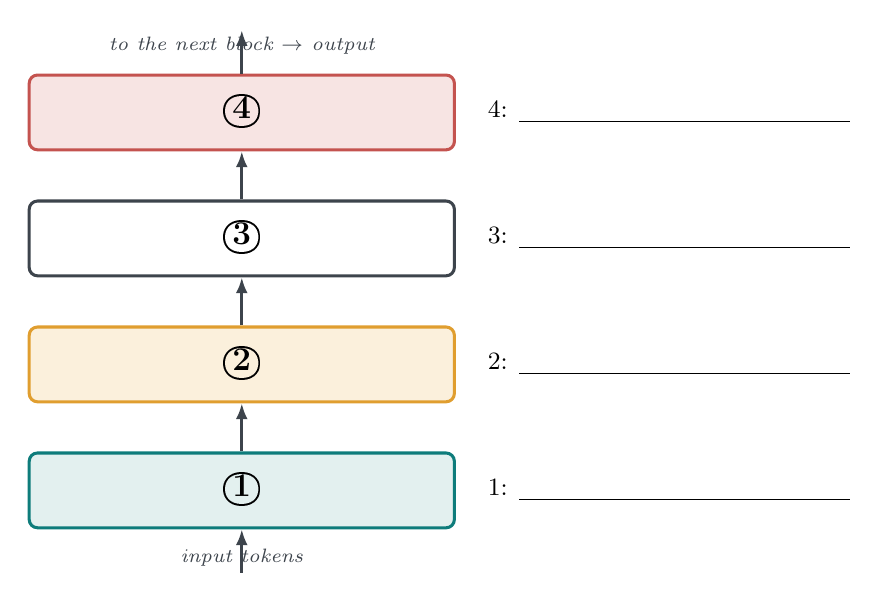
\begin{tikzpicture}[x=1cm, y=1cm, line join=round,
    blk/.style={rounded corners=3pt, draw, line width=1.1pt, minimum width=5.4cm,
                minimum height=0.95cm, align=center, font=\small\bfseries},
    ar/.style={-{Latex[length=2mm]}, line width=1pt, inksoft}]
  \node[blk, fill=tealsoft, draw=teal]   (b1) at (0,0)   {\large\textbf{\textcircled{1}}};
  \node[blk, fill=ambersoft, draw=amber] (b2) at (0,1.6) {\large\textbf{\textcircled{2}}};
  \node[blk, fill=white, draw=inksoft]   (b3) at (0,3.2) {\large\textbf{\textcircled{3}}};
  \node[blk, fill=redsoft, draw=redd]    (b4) at (0,4.8) {\large\textbf{\textcircled{4}}};
  \draw[ar] ($(b1.south)+(0,-0.55)$) -- (b1.south);
  \draw[ar] (b1.north) -- (b2.south);
  \draw[ar] (b2.north) -- (b3.south);
  \draw[ar] (b3.north) -- (b4.south);
  \draw[ar] (b4.north) -- ($(b4.north)+(0,0.55)$);
  \node[font=\scriptsize\itshape, inksoft] at (0,-0.85) {input tokens};
  \node[font=\scriptsize\itshape, inksoft] at (0,5.65) {to the next block $\rightarrow$ output};
  % answer lines to the right of each block
  \node[right, font=\small] at (3.0,0)   {1: \rb{Positional encoding}{4.2cm}};
  \node[right, font=\small] at (3.0,1.6) {2: \rb{Multi-head self-attention}{4.2cm}};
  \node[right, font=\small] at (3.0,3.2) {3: \rb{Add \& Norm (layer norm)}{4.2cm}};
  \node[right, font=\small] at (3.0,4.8) {4: \rb{Feed-forward network}{4.2cm}};
\end{tikzpicture}
\end{center}

\vspace{2pt}
\begin{center}
{\small \textbf{Word bank:}\;\; Feed-forward network \;$\cdot$\; Multi-head self-attention \;$\cdot$\;
Add \& Norm (layer norm) \;$\cdot$\; Positional encoding}
\end{center}

\keybox{Bottom to top: \textbf{1 = Positional encoding} (added to the input embeddings so attention can
see order), \textbf{2 = Multi-head self-attention} (the query/key/value weighted-average lookup),
\textbf{3 = Add \& Norm} (the residual skip plus layer normalization), \textbf{4 = Feed-forward network}
(a small per-token MLP). Attention comes before the feed-forward: attention mixes information \emph{across}
tokens, then the feed-forward refines each token on its own.}

\vspace{2pt}\hrule\vspace{5pt}

% =========================== Q2 ===========================
\textbf{2. Match each data type to a tokenization strategy.}\; {\small A transformer eats a sequence of
vectors, so MS data must be turned into tokens. Match each data type to the one strategy that fits it
best (each used once), using the decision chart from the slides.}

\vspace{4pt}
\textbf{(a)} An \textbf{imaging-MS image} (a 2D picture, one spectrum per pixel)\hfill
$\rightarrow$\;\rb{patches + linear projection (ViT)}{5.2cm}

\vspace{3pt}
\textbf{(b)} A \textbf{raw binned spectrum} (a dense 1D vector of $\sim$6{,}000 intensities)\hfill
$\rightarrow$\;\rb{CNN front-end}{5.2cm}

\vspace{3pt}
\textbf{(c)} A \textbf{peak list} (a sparse set of $m/z$ + intensity peaks)\hfill
$\rightarrow$\;\rb{peak-as-token (Casanovo)}{5.2cm}

\vspace{4pt}
\begin{center}
{\small \textbf{Word bank:}\;\; chunk into patches + linear projection (ViT) \;$\cdot$\;
CNN front-end \;$\cdot$\; peak-as-token (Casanovo)}
\end{center}

\keybox{(a) \textbf{Patches + linear projection (ViT-style)} --- a 2D image is cut into equal patches, each
projected to a token vector. (b) \textbf{CNN front-end} --- a dense, evenly-sampled 1D signal is best
condensed by a small 1D CNN that emits token embeddings (local peak-shape detection first, then the
transformer mixes globally). (c) \textbf{Peak-as-token} --- a sparse peak list is already a natural set of
tokens; each peak becomes one token carrying its $m/z$ and intensity, exactly how Casanovo reads a spectrum.}

\vspace{2pt}\hrule\vspace{5pt}

% =========================== Q3 ===========================
\textbf{3. Fine-tune, or train from scratch?}\; {\small You need a classifier for a new MS assay. You have
\textbf{800 labeled spectra}, and access to a transformer someone \textbf{pretrained on 2 million spectra}.}

\vspace{3pt}
\textbf{(a)} Would you \emph{train a new model from scratch} on your 800 spectra, or \emph{fine-tune} the
pretrained one?\hfill $\rightarrow$\;\rb{Fine-tune}{3.2cm}

\vspace{3pt}
\textbf{(b)} In one sentence, why?

\work{1.0cm}
\ifsolution\else\blk{\linewidth}\fi

\keybox{(a) \textbf{Fine-tune} --- freeze the pretrained body, bolt on a small new classification head, and
train mostly that head on the 800 labels (optionally unfreeze a little of the top with a much smaller
learning rate). (b) \textbf{800 labels are far too few to train a transformer's millions of weights from
scratch} --- it would overfit or collapse toward the majority class --- whereas \textbf{the pretrained body
already learned general spectral features from the 2 million spectra}, so you only need to fit a small head,
which 800 labels can do well. (Either reason earns full credit.)}

\vspace{2pt}\hrule\vspace{5pt}

% =========================== Q4 ===========================
\textbf{4. Which norm averages over what?}\; {\small Batch norm and layer norm both recenter values by
subtracting a mean --- but over \emph{different axes}. In the matrix below, \textbf{rows are tokens}
(samples in the batch) and \textbf{columns are features}.}

\vspace{4pt}
\begin{center}
\gr\begin{tabular}{r|G|G|G|}
\multicolumn{1}{r}{} & \multicolumn{1}{c}{\small f1} & \multicolumn{1}{c}{\small f2} & \multicolumn{1}{c}{\small f3}\\\cline{2-4}
\small tok1 & 2 & 4 & 6 \\\cline{2-4}
\small tok2 & 4 & 6 & 8 \\\cline{2-4}
\end{tabular}
\end{center}

\vspace{3pt}
\textbf{(a)} \textbf{Layer norm} averages across \rb{a token's features (one row)}{5.0cm}.\;
The layer-norm mean of \textbf{tok1} is\; $ (2+4+6)/3 = $ \rb{$4$}{1.6cm}

\work{0.5cm}

\textbf{(b)} \textbf{Batch norm} averages down \rb{a feature across the batch (one column)}{5.0cm}.\;
The batch-norm mean of feature \textbf{f1} is\; $ (2+4)/2 = $ \rb{$3$}{1.6cm}

\work{0.5cm}

\textbf{(c)} Give one reason \emph{transformers use layer norm} rather than batch norm.

\work{1.0cm}
\ifsolution\else\blk{\linewidth}\fi

\keybox{(a) Layer norm averages across \textbf{a token's own features (a row)} --- one mean per token ---
so tok1's mean is $(2+4+6)/3=\mathbf{4}$. (b) Batch norm averages down \textbf{a feature across the batch
(a column)} --- one mean per feature --- so f1's mean is $(2+4)/2=\mathbf{3}$. (c) \textbf{Layer norm needs
no batch statistics}: it looks only within a single token, so it is stable at batch size 1 and with
variable-length sequences (whereas batch norm's mean depends on the other samples in the batch) --- which
is exactly why transformers, whose inputs are ragged sequences, use it.}

\vspace{4pt}\hrule\vspace{3pt}
{\small\itshape \ifsolution Answer key.\else Keep this sheet --- Lab 3 fine-tunes a real pretrained
transformer, freezing the body and training a new head.\fi}

\end{document}
"
%  (or, to flip by hand, change \solutionfalse to \solutiontrue below.)
% =====================================================================
\documentclass[11pt]{article}

\newif\ifsolution
\ifdefined\showsolutions \solutiontrue \else \solutionfalse \fi
% \solutiontrue   % <-- uncomment to hard-code the ANSWER KEY build

\usepackage[letterpaper, margin=0.6in, top=0.7in, bottom=0.5in]{geometry}
\usepackage{amsmath, amssymb}
\usepackage{xcolor}
\usepackage{array}
\usepackage{tikz}
\usetikzlibrary{arrows.meta, calc}
\usepackage{fancyhdr}

\pagestyle{fancy}
\fancyhf{}
\fancyhead[L]{\small\textbf{MSACL DS301 --- Deep Learning}}
\fancyhead[R]{\small\textbf{Quiz 8: The Transformer, Assembled\ifsolution\ \textmd{(Answer Key)}\fi}}
\fancyfoot[C]{\thepage}
\renewcommand{\headrulewidth}{0.4pt}

\newcommand{\blk}[1]{\underline{\hspace{#1}}}
% Reveal-or-blank: shows the answer in the key, a blank rule on the student sheet.
\newcommand{\rb}[2]{\ifsolution\textbf{#1}\else\blk{#2}\fi}
% Boxed answer (key only) and blank writing space (student only).
\newcommand{\keybox}[1]{\ifsolution\par\vspace{2pt}%
  \fbox{\parbox{0.965\textwidth}{\small\textbf{Answer.}\; #1}}\par\fi}
\newcommand{\work}[1]{\ifsolution\else\vspace{#1}\fi}

% ---- course palette (numeric grids / diagram) ----------------------------
\definecolor{ink}{HTML}{1B2025}
\definecolor{teal}{HTML}{0E7C7B}
\definecolor{tealsoft}{HTML}{E3F0EF}
\definecolor{amber}{HTML}{E09E2F}
\definecolor{ambersoft}{HTML}{FBF0DC}
\definecolor{redd}{HTML}{C4534F}
\definecolor{redsoft}{HTML}{F7E4E3}
\definecolor{inksoft}{HTML}{3D444C}
% square, centred, monospace cells for the numeric grids
\newcolumntype{G}{>{\centering\arraybackslash\ttfamily}p{7mm}}
\newcommand{\gr}{\renewcommand{\arraystretch}{1.5}}

\setlength{\parindent}{0pt}
\setlength{\parskip}{3pt}
\setlength{\abovedisplayskip}{5pt}
\setlength{\belowdisplayskip}{5pt}

\begin{document}

\begin{center}
{\Large \textbf{Quiz 8 --- The Transformer, Assembled}}\\[2pt]
{\normalsize Label the blocks, match a spectrum to its tokens, fine-tune or not, and which norm averages what}
\end{center}

\vspace{-2pt}
\begin{center}
\fbox{\parbox{0.92\textwidth}{\small
\textbf{Instructions:}\; Answer all four questions --- every part is answerable from the diagrams and
rules on the slides. Intuition first; the only arithmetic is a mean. No calculators needed.%
\ifsolution\else\\[4pt]\textbf{Name:}\ \blk{6cm}\hfill\textbf{Date:}\ \blk{3.5cm}\fi
}}
\end{center}

\vspace{-2pt}\hrule\vspace{5pt}

% =========================== Q1 ===========================
\textbf{1. Label the four transformer blocks.}\; {\small Below is one transformer (encoder) block,
read bottom to top --- the same block you labelled on the slides, now blank. Write the name of each
numbered block on the line beside it, using the word bank.}

\vspace{4pt}
\begin{center}
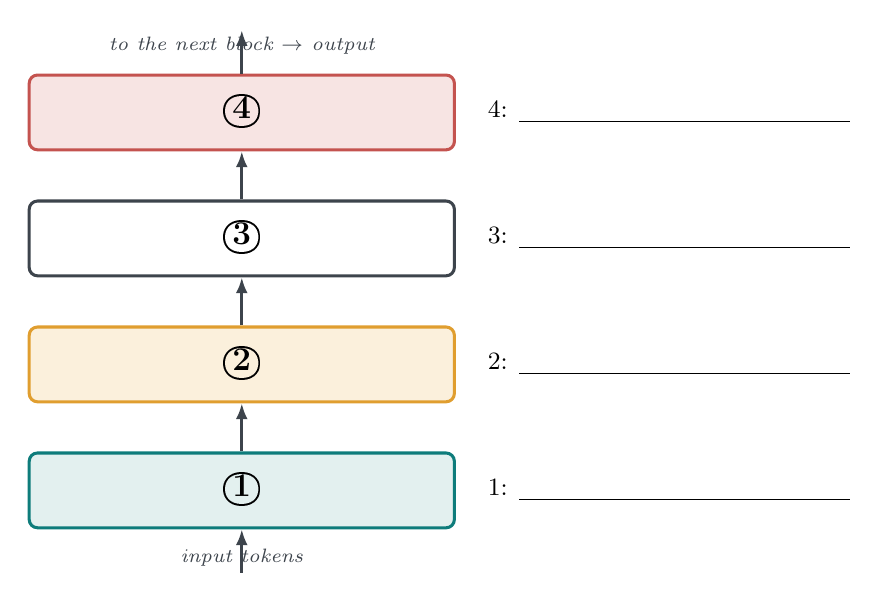
\begin{tikzpicture}[x=1cm, y=1cm, line join=round,
    blk/.style={rounded corners=3pt, draw, line width=1.1pt, minimum width=5.4cm,
                minimum height=0.95cm, align=center, font=\small\bfseries},
    ar/.style={-{Latex[length=2mm]}, line width=1pt, inksoft}]
  \node[blk, fill=tealsoft, draw=teal]   (b1) at (0,0)   {\large\textbf{\textcircled{1}}};
  \node[blk, fill=ambersoft, draw=amber] (b2) at (0,1.6) {\large\textbf{\textcircled{2}}};
  \node[blk, fill=white, draw=inksoft]   (b3) at (0,3.2) {\large\textbf{\textcircled{3}}};
  \node[blk, fill=redsoft, draw=redd]    (b4) at (0,4.8) {\large\textbf{\textcircled{4}}};
  \draw[ar] ($(b1.south)+(0,-0.55)$) -- (b1.south);
  \draw[ar] (b1.north) -- (b2.south);
  \draw[ar] (b2.north) -- (b3.south);
  \draw[ar] (b3.north) -- (b4.south);
  \draw[ar] (b4.north) -- ($(b4.north)+(0,0.55)$);
  \node[font=\scriptsize\itshape, inksoft] at (0,-0.85) {input tokens};
  \node[font=\scriptsize\itshape, inksoft] at (0,5.65) {to the next block $\rightarrow$ output};
  % answer lines to the right of each block
  \node[right, font=\small] at (3.0,0)   {1: \rb{Positional encoding}{4.2cm}};
  \node[right, font=\small] at (3.0,1.6) {2: \rb{Multi-head self-attention}{4.2cm}};
  \node[right, font=\small] at (3.0,3.2) {3: \rb{Add \& Norm (layer norm)}{4.2cm}};
  \node[right, font=\small] at (3.0,4.8) {4: \rb{Feed-forward network}{4.2cm}};
\end{tikzpicture}
\end{center}

\vspace{2pt}
\begin{center}
{\small \textbf{Word bank:}\;\; Feed-forward network \;$\cdot$\; Multi-head self-attention \;$\cdot$\;
Add \& Norm (layer norm) \;$\cdot$\; Positional encoding}
\end{center}

\keybox{Bottom to top: \textbf{1 = Positional encoding} (added to the input embeddings so attention can
see order), \textbf{2 = Multi-head self-attention} (the query/key/value weighted-average lookup),
\textbf{3 = Add \& Norm} (the residual skip plus layer normalization), \textbf{4 = Feed-forward network}
(a small per-token MLP). Attention comes before the feed-forward: attention mixes information \emph{across}
tokens, then the feed-forward refines each token on its own.}

\vspace{2pt}\hrule\vspace{5pt}

% =========================== Q2 ===========================
\textbf{2. Match each data type to a tokenization strategy.}\; {\small A transformer eats a sequence of
vectors, so MS data must be turned into tokens. Match each data type to the one strategy that fits it
best (each used once), using the decision chart from the slides.}

\vspace{4pt}
\textbf{(a)} An \textbf{imaging-MS image} (a 2D picture, one spectrum per pixel)\hfill
$\rightarrow$\;\rb{patches + linear projection (ViT)}{5.2cm}

\vspace{3pt}
\textbf{(b)} A \textbf{raw binned spectrum} (a dense 1D vector of $\sim$6{,}000 intensities)\hfill
$\rightarrow$\;\rb{CNN front-end}{5.2cm}

\vspace{3pt}
\textbf{(c)} A \textbf{peak list} (a sparse set of $m/z$ + intensity peaks)\hfill
$\rightarrow$\;\rb{peak-as-token (Casanovo)}{5.2cm}

\vspace{4pt}
\begin{center}
{\small \textbf{Word bank:}\;\; chunk into patches + linear projection (ViT) \;$\cdot$\;
CNN front-end \;$\cdot$\; peak-as-token (Casanovo)}
\end{center}

\keybox{(a) \textbf{Patches + linear projection (ViT-style)} --- a 2D image is cut into equal patches, each
projected to a token vector. (b) \textbf{CNN front-end} --- a dense, evenly-sampled 1D signal is best
condensed by a small 1D CNN that emits token embeddings (local peak-shape detection first, then the
transformer mixes globally). (c) \textbf{Peak-as-token} --- a sparse peak list is already a natural set of
tokens; each peak becomes one token carrying its $m/z$ and intensity, exactly how Casanovo reads a spectrum.}

\vspace{2pt}\hrule\vspace{5pt}

% =========================== Q3 ===========================
\textbf{3. Fine-tune, or train from scratch?}\; {\small You need a classifier for a new MS assay. You have
\textbf{800 labeled spectra}, and access to a transformer someone \textbf{pretrained on 2 million spectra}.}

\vspace{3pt}
\textbf{(a)} Would you \emph{train a new model from scratch} on your 800 spectra, or \emph{fine-tune} the
pretrained one?\hfill $\rightarrow$\;\rb{Fine-tune}{3.2cm}

\vspace{3pt}
\textbf{(b)} In one sentence, why?

\work{1.0cm}
\ifsolution\else\blk{\linewidth}\fi

\keybox{(a) \textbf{Fine-tune} --- freeze the pretrained body, bolt on a small new classification head, and
train mostly that head on the 800 labels (optionally unfreeze a little of the top with a much smaller
learning rate). (b) \textbf{800 labels are far too few to train a transformer's millions of weights from
scratch} --- it would overfit or collapse toward the majority class --- whereas \textbf{the pretrained body
already learned general spectral features from the 2 million spectra}, so you only need to fit a small head,
which 800 labels can do well. (Either reason earns full credit.)}

\vspace{2pt}\hrule\vspace{5pt}

% =========================== Q4 ===========================
\textbf{4. Which norm averages over what?}\; {\small Batch norm and layer norm both recenter values by
subtracting a mean --- but over \emph{different axes}. In the matrix below, \textbf{rows are tokens}
(samples in the batch) and \textbf{columns are features}.}

\vspace{4pt}
\begin{center}
\gr\begin{tabular}{r|G|G|G|}
\multicolumn{1}{r}{} & \multicolumn{1}{c}{\small f1} & \multicolumn{1}{c}{\small f2} & \multicolumn{1}{c}{\small f3}\\\cline{2-4}
\small tok1 & 2 & 4 & 6 \\\cline{2-4}
\small tok2 & 4 & 6 & 8 \\\cline{2-4}
\end{tabular}
\end{center}

\vspace{3pt}
\textbf{(a)} \textbf{Layer norm} averages across \rb{a token's features (one row)}{5.0cm}.\;
The layer-norm mean of \textbf{tok1} is\; $ (2+4+6)/3 = $ \rb{$4$}{1.6cm}

\work{0.5cm}

\textbf{(b)} \textbf{Batch norm} averages down \rb{a feature across the batch (one column)}{5.0cm}.\;
The batch-norm mean of feature \textbf{f1} is\; $ (2+4)/2 = $ \rb{$3$}{1.6cm}

\work{0.5cm}

\textbf{(c)} Give one reason \emph{transformers use layer norm} rather than batch norm.

\work{1.0cm}
\ifsolution\else\blk{\linewidth}\fi

\keybox{(a) Layer norm averages across \textbf{a token's own features (a row)} --- one mean per token ---
so tok1's mean is $(2+4+6)/3=\mathbf{4}$. (b) Batch norm averages down \textbf{a feature across the batch
(a column)} --- one mean per feature --- so f1's mean is $(2+4)/2=\mathbf{3}$. (c) \textbf{Layer norm needs
no batch statistics}: it looks only within a single token, so it is stable at batch size 1 and with
variable-length sequences (whereas batch norm's mean depends on the other samples in the batch) --- which
is exactly why transformers, whose inputs are ragged sequences, use it.}

\vspace{4pt}\hrule\vspace{3pt}
{\small\itshape \ifsolution Answer key.\else Keep this sheet --- Lab 3 fine-tunes a real pretrained
transformer, freezing the body and training a new head.\fi}

\end{document}
"
%  (or, to flip by hand, change \solutionfalse to \solutiontrue below.)
% =====================================================================
\documentclass[11pt]{article}

\newif\ifsolution
\ifdefined\showsolutions \solutiontrue \else \solutionfalse \fi
% \solutiontrue   % <-- uncomment to hard-code the ANSWER KEY build

\usepackage[letterpaper, margin=0.6in, top=0.7in, bottom=0.5in]{geometry}
\usepackage{amsmath, amssymb}
\usepackage{xcolor}
\usepackage{array}
\usepackage{tikz}
\usetikzlibrary{arrows.meta, calc}
\usepackage{fancyhdr}

\pagestyle{fancy}
\fancyhf{}
\fancyhead[L]{\small\textbf{MSACL DS301 --- Deep Learning}}
\fancyhead[R]{\small\textbf{Quiz 8: The Transformer, Assembled\ifsolution\ \textmd{(Answer Key)}\fi}}
\fancyfoot[C]{\thepage}
\renewcommand{\headrulewidth}{0.4pt}

\newcommand{\blk}[1]{\underline{\hspace{#1}}}
% Reveal-or-blank: shows the answer in the key, a blank rule on the student sheet.
\newcommand{\rb}[2]{\ifsolution\textbf{#1}\else\blk{#2}\fi}
% Boxed answer (key only) and blank writing space (student only).
\newcommand{\keybox}[1]{\ifsolution\par\vspace{2pt}%
  \fbox{\parbox{0.965\textwidth}{\small\textbf{Answer.}\; #1}}\par\fi}
\newcommand{\work}[1]{\ifsolution\else\vspace{#1}\fi}

% ---- course palette (numeric grids / diagram) ----------------------------
\definecolor{ink}{HTML}{1B2025}
\definecolor{teal}{HTML}{0E7C7B}
\definecolor{tealsoft}{HTML}{E3F0EF}
\definecolor{amber}{HTML}{E09E2F}
\definecolor{ambersoft}{HTML}{FBF0DC}
\definecolor{redd}{HTML}{C4534F}
\definecolor{redsoft}{HTML}{F7E4E3}
\definecolor{inksoft}{HTML}{3D444C}
% square, centred, monospace cells for the numeric grids
\newcolumntype{G}{>{\centering\arraybackslash\ttfamily}p{7mm}}
\newcommand{\gr}{\renewcommand{\arraystretch}{1.5}}

\setlength{\parindent}{0pt}
\setlength{\parskip}{3pt}
\setlength{\abovedisplayskip}{5pt}
\setlength{\belowdisplayskip}{5pt}

\begin{document}

\begin{center}
{\Large \textbf{Quiz 8 --- The Transformer, Assembled}}\\[2pt]
{\normalsize Label the blocks, match a spectrum to its tokens, fine-tune or not, and which norm averages what}
\end{center}

\vspace{-2pt}
\begin{center}
\fbox{\parbox{0.92\textwidth}{\small
\textbf{Instructions:}\; Answer all four questions --- every part is answerable from the diagrams and
rules on the slides. Intuition first; the only arithmetic is a mean. No calculators needed.%
\ifsolution\else\\[4pt]\textbf{Name:}\ \blk{6cm}\hfill\textbf{Date:}\ \blk{3.5cm}\fi
}}
\end{center}

\vspace{-2pt}\hrule\vspace{5pt}

% =========================== Q1 ===========================
\textbf{1. Label the four transformer blocks.}\; {\small Below is one transformer (encoder) block,
read bottom to top --- the same block you labelled on the slides, now blank. Write the name of each
numbered block on the line beside it, using the word bank.}

\vspace{4pt}
\begin{center}
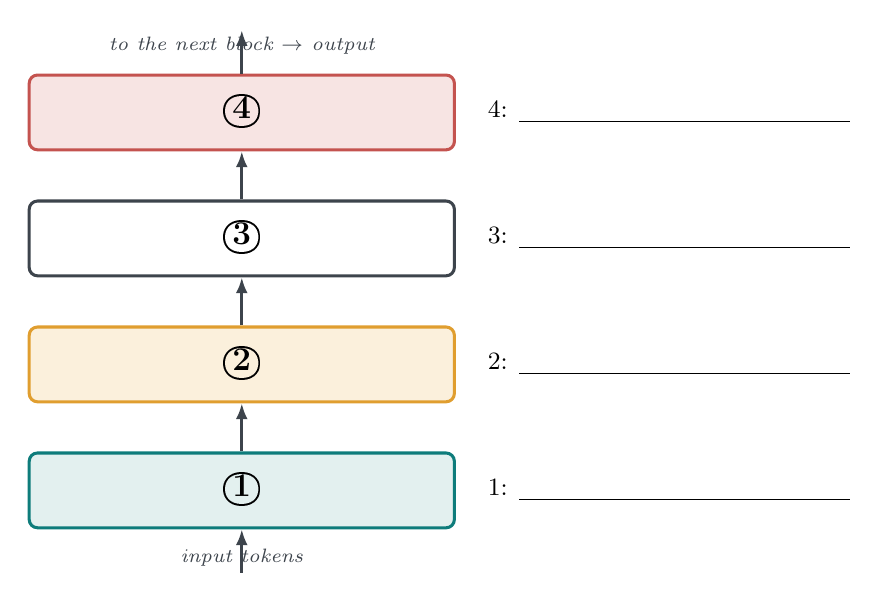
\begin{tikzpicture}[x=1cm, y=1cm, line join=round,
    blk/.style={rounded corners=3pt, draw, line width=1.1pt, minimum width=5.4cm,
                minimum height=0.95cm, align=center, font=\small\bfseries},
    ar/.style={-{Latex[length=2mm]}, line width=1pt, inksoft}]
  \node[blk, fill=tealsoft, draw=teal]   (b1) at (0,0)   {\large\textbf{\textcircled{1}}};
  \node[blk, fill=ambersoft, draw=amber] (b2) at (0,1.6) {\large\textbf{\textcircled{2}}};
  \node[blk, fill=white, draw=inksoft]   (b3) at (0,3.2) {\large\textbf{\textcircled{3}}};
  \node[blk, fill=redsoft, draw=redd]    (b4) at (0,4.8) {\large\textbf{\textcircled{4}}};
  \draw[ar] ($(b1.south)+(0,-0.55)$) -- (b1.south);
  \draw[ar] (b1.north) -- (b2.south);
  \draw[ar] (b2.north) -- (b3.south);
  \draw[ar] (b3.north) -- (b4.south);
  \draw[ar] (b4.north) -- ($(b4.north)+(0,0.55)$);
  \node[font=\scriptsize\itshape, inksoft] at (0,-0.85) {input tokens};
  \node[font=\scriptsize\itshape, inksoft] at (0,5.65) {to the next block $\rightarrow$ output};
  % answer lines to the right of each block
  \node[right, font=\small] at (3.0,0)   {1: \rb{Positional encoding}{4.2cm}};
  \node[right, font=\small] at (3.0,1.6) {2: \rb{Multi-head self-attention}{4.2cm}};
  \node[right, font=\small] at (3.0,3.2) {3: \rb{Add \& Norm (layer norm)}{4.2cm}};
  \node[right, font=\small] at (3.0,4.8) {4: \rb{Feed-forward network}{4.2cm}};
\end{tikzpicture}
\end{center}

\vspace{2pt}
\begin{center}
{\small \textbf{Word bank:}\;\; Feed-forward network \;$\cdot$\; Multi-head self-attention \;$\cdot$\;
Add \& Norm (layer norm) \;$\cdot$\; Positional encoding}
\end{center}

\keybox{Bottom to top: \textbf{1 = Positional encoding} (added to the input embeddings so attention can
see order), \textbf{2 = Multi-head self-attention} (the query/key/value weighted-average lookup),
\textbf{3 = Add \& Norm} (the residual skip plus layer normalization), \textbf{4 = Feed-forward network}
(a small per-token MLP). Attention comes before the feed-forward: attention mixes information \emph{across}
tokens, then the feed-forward refines each token on its own.}

\vspace{2pt}\hrule\vspace{5pt}

% =========================== Q2 ===========================
\textbf{2. Match each data type to a tokenization strategy.}\; {\small A transformer eats a sequence of
vectors, so MS data must be turned into tokens. Match each data type to the one strategy that fits it
best (each used once), using the decision chart from the slides.}

\vspace{4pt}
\textbf{(a)} An \textbf{imaging-MS image} (a 2D picture, one spectrum per pixel)\hfill
$\rightarrow$\;\rb{patches + linear projection (ViT)}{5.2cm}

\vspace{3pt}
\textbf{(b)} A \textbf{raw binned spectrum} (a dense 1D vector of $\sim$6{,}000 intensities)\hfill
$\rightarrow$\;\rb{CNN front-end}{5.2cm}

\vspace{3pt}
\textbf{(c)} A \textbf{peak list} (a sparse set of $m/z$ + intensity peaks)\hfill
$\rightarrow$\;\rb{peak-as-token (Casanovo)}{5.2cm}

\vspace{4pt}
\begin{center}
{\small \textbf{Word bank:}\;\; chunk into patches + linear projection (ViT) \;$\cdot$\;
CNN front-end \;$\cdot$\; peak-as-token (Casanovo)}
\end{center}

\keybox{(a) \textbf{Patches + linear projection (ViT-style)} --- a 2D image is cut into equal patches, each
projected to a token vector. (b) \textbf{CNN front-end} --- a dense, evenly-sampled 1D signal is best
condensed by a small 1D CNN that emits token embeddings (local peak-shape detection first, then the
transformer mixes globally). (c) \textbf{Peak-as-token} --- a sparse peak list is already a natural set of
tokens; each peak becomes one token carrying its $m/z$ and intensity, exactly how Casanovo reads a spectrum.}

\vspace{2pt}\hrule\vspace{5pt}

% =========================== Q3 ===========================
\textbf{3. Fine-tune, or train from scratch?}\; {\small You need a classifier for a new MS assay. You have
\textbf{800 labeled spectra}, and access to a transformer someone \textbf{pretrained on 2 million spectra}.}

\vspace{3pt}
\textbf{(a)} Would you \emph{train a new model from scratch} on your 800 spectra, or \emph{fine-tune} the
pretrained one?\hfill $\rightarrow$\;\rb{Fine-tune}{3.2cm}

\vspace{3pt}
\textbf{(b)} In one sentence, why?

\work{1.0cm}
\ifsolution\else\blk{\linewidth}\fi

\keybox{(a) \textbf{Fine-tune} --- freeze the pretrained body, bolt on a small new classification head, and
train mostly that head on the 800 labels (optionally unfreeze a little of the top with a much smaller
learning rate). (b) \textbf{800 labels are far too few to train a transformer's millions of weights from
scratch} --- it would overfit or collapse toward the majority class --- whereas \textbf{the pretrained body
already learned general spectral features from the 2 million spectra}, so you only need to fit a small head,
which 800 labels can do well. (Either reason earns full credit.)}

\vspace{2pt}\hrule\vspace{5pt}

% =========================== Q4 ===========================
\textbf{4. Which norm averages over what?}\; {\small Batch norm and layer norm both recenter values by
subtracting a mean --- but over \emph{different axes}. In the matrix below, \textbf{rows are tokens}
(samples in the batch) and \textbf{columns are features}.}

\vspace{4pt}
\begin{center}
\gr\begin{tabular}{r|G|G|G|}
\multicolumn{1}{r}{} & \multicolumn{1}{c}{\small f1} & \multicolumn{1}{c}{\small f2} & \multicolumn{1}{c}{\small f3}\\\cline{2-4}
\small tok1 & 2 & 4 & 6 \\\cline{2-4}
\small tok2 & 4 & 6 & 8 \\\cline{2-4}
\end{tabular}
\end{center}

\vspace{3pt}
\textbf{(a)} \textbf{Layer norm} averages across \rb{a token's features (one row)}{5.0cm}.\;
The layer-norm mean of \textbf{tok1} is\; $ (2+4+6)/3 = $ \rb{$4$}{1.6cm}

\work{0.5cm}

\textbf{(b)} \textbf{Batch norm} averages down \rb{a feature across the batch (one column)}{5.0cm}.\;
The batch-norm mean of feature \textbf{f1} is\; $ (2+4)/2 = $ \rb{$3$}{1.6cm}

\work{0.5cm}

\textbf{(c)} Give one reason \emph{transformers use layer norm} rather than batch norm.

\work{1.0cm}
\ifsolution\else\blk{\linewidth}\fi

\keybox{(a) Layer norm averages across \textbf{a token's own features (a row)} --- one mean per token ---
so tok1's mean is $(2+4+6)/3=\mathbf{4}$. (b) Batch norm averages down \textbf{a feature across the batch
(a column)} --- one mean per feature --- so f1's mean is $(2+4)/2=\mathbf{3}$. (c) \textbf{Layer norm needs
no batch statistics}: it looks only within a single token, so it is stable at batch size 1 and with
variable-length sequences (whereas batch norm's mean depends on the other samples in the batch) --- which
is exactly why transformers, whose inputs are ragged sequences, use it.}

\vspace{4pt}\hrule\vspace{3pt}
{\small\itshape \ifsolution Answer key.\else Keep this sheet --- Lab 3 fine-tunes a real pretrained
transformer, freezing the body and training a new head.\fi}

\end{document}
"
%  (or, to flip by hand, change \solutionfalse to \solutiontrue below.)
% =====================================================================
\documentclass[11pt]{article}

\newif\ifsolution
\ifdefined\showsolutions \solutiontrue \else \solutionfalse \fi
% \solutiontrue   % <-- uncomment to hard-code the ANSWER KEY build

\usepackage[letterpaper, margin=0.6in, top=0.7in, bottom=0.5in]{geometry}
\usepackage{amsmath, amssymb}
\usepackage{xcolor}
\usepackage{array}
\usepackage{tikz}
\usetikzlibrary{arrows.meta, calc}
\usepackage{fancyhdr}

\pagestyle{fancy}
\fancyhf{}
\fancyhead[L]{\small\textbf{MSACL DS301 --- Deep Learning}}
\fancyhead[R]{\small\textbf{Quiz 8: The Transformer, Assembled\ifsolution\ \textmd{(Answer Key)}\fi}}
\fancyfoot[C]{\thepage}
\renewcommand{\headrulewidth}{0.4pt}

\newcommand{\blk}[1]{\underline{\hspace{#1}}}
% Reveal-or-blank: shows the answer in the key, a blank rule on the student sheet.
\newcommand{\rb}[2]{\ifsolution\textbf{#1}\else\blk{#2}\fi}
% Boxed answer (key only) and blank writing space (student only).
\newcommand{\keybox}[1]{\ifsolution\par\vspace{2pt}%
  \fbox{\parbox{0.965\textwidth}{\small\textbf{Answer.}\; #1}}\par\fi}
\newcommand{\work}[1]{\ifsolution\else\vspace{#1}\fi}

% ---- course palette (numeric grids / diagram) ----------------------------
\definecolor{ink}{HTML}{1B2025}
\definecolor{teal}{HTML}{0E7C7B}
\definecolor{tealsoft}{HTML}{E3F0EF}
\definecolor{amber}{HTML}{E09E2F}
\definecolor{ambersoft}{HTML}{FBF0DC}
\definecolor{redd}{HTML}{C4534F}
\definecolor{redsoft}{HTML}{F7E4E3}
\definecolor{inksoft}{HTML}{3D444C}
% square, centred, monospace cells for the numeric grids
\newcolumntype{G}{>{\centering\arraybackslash\ttfamily}p{7mm}}
\newcommand{\gr}{\renewcommand{\arraystretch}{1.5}}

\setlength{\parindent}{0pt}
\setlength{\parskip}{3pt}
\setlength{\abovedisplayskip}{5pt}
\setlength{\belowdisplayskip}{5pt}

\begin{document}

\begin{center}
{\Large \textbf{Quiz 8 --- The Transformer, Assembled}}\\[2pt]
{\normalsize Label the blocks, match a spectrum to its tokens, fine-tune or not, and which norm averages what}
\end{center}

\vspace{-2pt}
\begin{center}
\fbox{\parbox{0.92\textwidth}{\small
\textbf{Instructions:}\; Answer all four questions --- every part is answerable from the diagrams and
rules on the slides. Intuition first; the only arithmetic is a mean. No calculators needed.%
\ifsolution\else\\[4pt]\textbf{Name:}\ \blk{6cm}\hfill\textbf{Date:}\ \blk{3.5cm}\fi
}}
\end{center}

\vspace{-2pt}\hrule\vspace{5pt}

% =========================== Q1 ===========================
\textbf{1. Label the four transformer blocks.}\; {\small Below is one transformer (encoder) block,
read bottom to top --- the same block you labelled on the slides, now blank. Write the name of each
numbered block on the line beside it, using the word bank.}

\vspace{4pt}
\begin{center}
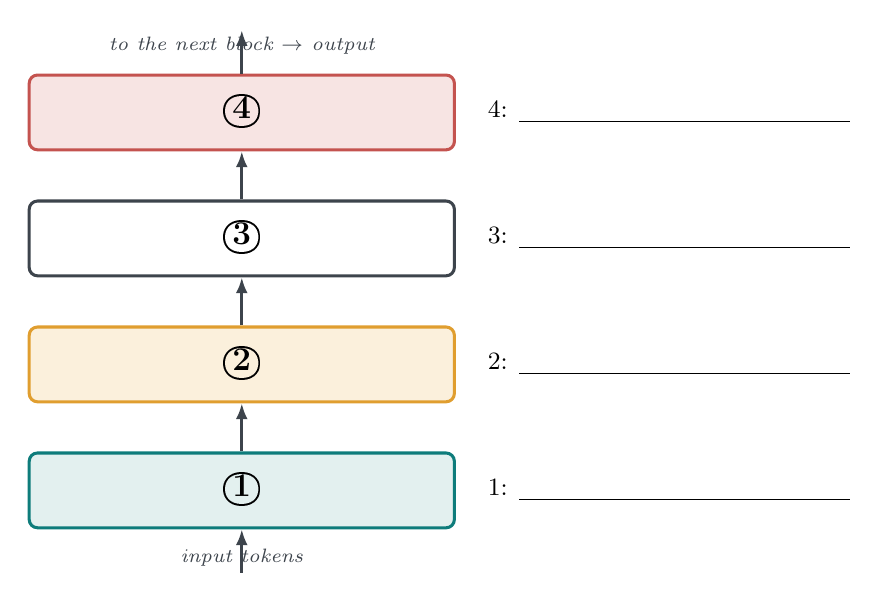
\begin{tikzpicture}[x=1cm, y=1cm, line join=round,
    blk/.style={rounded corners=3pt, draw, line width=1.1pt, minimum width=5.4cm,
                minimum height=0.95cm, align=center, font=\small\bfseries},
    ar/.style={-{Latex[length=2mm]}, line width=1pt, inksoft}]
  \node[blk, fill=tealsoft, draw=teal]   (b1) at (0,0)   {\large\textbf{\textcircled{1}}};
  \node[blk, fill=ambersoft, draw=amber] (b2) at (0,1.6) {\large\textbf{\textcircled{2}}};
  \node[blk, fill=white, draw=inksoft]   (b3) at (0,3.2) {\large\textbf{\textcircled{3}}};
  \node[blk, fill=redsoft, draw=redd]    (b4) at (0,4.8) {\large\textbf{\textcircled{4}}};
  \draw[ar] ($(b1.south)+(0,-0.55)$) -- (b1.south);
  \draw[ar] (b1.north) -- (b2.south);
  \draw[ar] (b2.north) -- (b3.south);
  \draw[ar] (b3.north) -- (b4.south);
  \draw[ar] (b4.north) -- ($(b4.north)+(0,0.55)$);
  \node[font=\scriptsize\itshape, inksoft] at (0,-0.85) {input tokens};
  \node[font=\scriptsize\itshape, inksoft] at (0,5.65) {to the next block $\rightarrow$ output};
  % answer lines to the right of each block
  \node[right, font=\small] at (3.0,0)   {1: \rb{Positional encoding}{4.2cm}};
  \node[right, font=\small] at (3.0,1.6) {2: \rb{Multi-head self-attention}{4.2cm}};
  \node[right, font=\small] at (3.0,3.2) {3: \rb{Add \& Norm (layer norm)}{4.2cm}};
  \node[right, font=\small] at (3.0,4.8) {4: \rb{Feed-forward network}{4.2cm}};
\end{tikzpicture}
\end{center}

\vspace{2pt}
\begin{center}
{\small \textbf{Word bank:}\;\; Feed-forward network \;$\cdot$\; Multi-head self-attention \;$\cdot$\;
Add \& Norm (layer norm) \;$\cdot$\; Positional encoding}
\end{center}

\keybox{Bottom to top: \textbf{1 = Positional encoding} (added to the input embeddings so attention can
see order), \textbf{2 = Multi-head self-attention} (the query/key/value weighted-average lookup),
\textbf{3 = Add \& Norm} (the residual skip plus layer normalization), \textbf{4 = Feed-forward network}
(a small per-token MLP). Attention comes before the feed-forward: attention mixes information \emph{across}
tokens, then the feed-forward refines each token on its own.}

\vspace{2pt}\hrule\vspace{5pt}

% =========================== Q2 ===========================
\textbf{2. Match each data type to a tokenization strategy.}\; {\small A transformer eats a sequence of
vectors, so MS data must be turned into tokens. Match each data type to the one strategy that fits it
best (each used once), using the decision chart from the slides.}

\vspace{4pt}
\textbf{(a)} An \textbf{imaging-MS image} (a 2D picture, one spectrum per pixel)\hfill
$\rightarrow$\;\rb{patches + linear projection (ViT)}{5.2cm}

\vspace{3pt}
\textbf{(b)} A \textbf{raw binned spectrum} (a dense 1D vector of $\sim$6{,}000 intensities)\hfill
$\rightarrow$\;\rb{CNN front-end}{5.2cm}

\vspace{3pt}
\textbf{(c)} A \textbf{peak list} (a sparse set of $m/z$ + intensity peaks)\hfill
$\rightarrow$\;\rb{peak-as-token (Casanovo)}{5.2cm}

\vspace{4pt}
\begin{center}
{\small \textbf{Word bank:}\;\; chunk into patches + linear projection (ViT) \;$\cdot$\;
CNN front-end \;$\cdot$\; peak-as-token (Casanovo)}
\end{center}

\keybox{(a) \textbf{Patches + linear projection (ViT-style)} --- a 2D image is cut into equal patches, each
projected to a token vector. (b) \textbf{CNN front-end} --- a dense, evenly-sampled 1D signal is best
condensed by a small 1D CNN that emits token embeddings (local peak-shape detection first, then the
transformer mixes globally). (c) \textbf{Peak-as-token} --- a sparse peak list is already a natural set of
tokens; each peak becomes one token carrying its $m/z$ and intensity, exactly how Casanovo reads a spectrum.}

\vspace{2pt}\hrule\vspace{5pt}

% =========================== Q3 ===========================
\textbf{3. Fine-tune, or train from scratch?}\; {\small You need a classifier for a new MS assay. You have
\textbf{800 labeled spectra}, and access to a transformer someone \textbf{pretrained on 2 million spectra}.}

\vspace{3pt}
\textbf{(a)} Would you \emph{train a new model from scratch} on your 800 spectra, or \emph{fine-tune} the
pretrained one?\hfill $\rightarrow$\;\rb{Fine-tune}{3.2cm}

\vspace{3pt}
\textbf{(b)} In one sentence, why?

\work{1.0cm}
\ifsolution\else\blk{\linewidth}\fi

\keybox{(a) \textbf{Fine-tune} --- freeze the pretrained body, bolt on a small new classification head, and
train mostly that head on the 800 labels (optionally unfreeze a little of the top with a much smaller
learning rate). (b) \textbf{800 labels are far too few to train a transformer's millions of weights from
scratch} --- it would overfit or collapse toward the majority class --- whereas \textbf{the pretrained body
already learned general spectral features from the 2 million spectra}, so you only need to fit a small head,
which 800 labels can do well. (Either reason earns full credit.)}

\vspace{2pt}\hrule\vspace{5pt}

% =========================== Q4 ===========================
\textbf{4. Which norm averages over what?}\; {\small Batch norm and layer norm both recenter values by
subtracting a mean --- but over \emph{different axes}. In the matrix below, \textbf{rows are tokens}
(samples in the batch) and \textbf{columns are features}.}

\vspace{4pt}
\begin{center}
\gr\begin{tabular}{r|G|G|G|}
\multicolumn{1}{r}{} & \multicolumn{1}{c}{\small f1} & \multicolumn{1}{c}{\small f2} & \multicolumn{1}{c}{\small f3}\\\cline{2-4}
\small tok1 & 2 & 4 & 6 \\\cline{2-4}
\small tok2 & 4 & 6 & 8 \\\cline{2-4}
\end{tabular}
\end{center}

\vspace{3pt}
\textbf{(a)} \textbf{Layer norm} averages across \rb{a token's features (one row)}{5.0cm}.\;
The layer-norm mean of \textbf{tok1} is\; $ (2+4+6)/3 = $ \rb{$4$}{1.6cm}

\work{0.5cm}

\textbf{(b)} \textbf{Batch norm} averages down \rb{a feature across the batch (one column)}{5.0cm}.\;
The batch-norm mean of feature \textbf{f1} is\; $ (2+4)/2 = $ \rb{$3$}{1.6cm}

\work{0.5cm}

\textbf{(c)} Give one reason \emph{transformers use layer norm} rather than batch norm.

\work{1.0cm}
\ifsolution\else\blk{\linewidth}\fi

\keybox{(a) Layer norm averages across \textbf{a token's own features (a row)} --- one mean per token ---
so tok1's mean is $(2+4+6)/3=\mathbf{4}$. (b) Batch norm averages down \textbf{a feature across the batch
(a column)} --- one mean per feature --- so f1's mean is $(2+4)/2=\mathbf{3}$. (c) \textbf{Layer norm needs
no batch statistics}: it looks only within a single token, so it is stable at batch size 1 and with
variable-length sequences (whereas batch norm's mean depends on the other samples in the batch) --- which
is exactly why transformers, whose inputs are ragged sequences, use it.}

\vspace{4pt}\hrule\vspace{3pt}
{\small\itshape \ifsolution Answer key.\else Keep this sheet --- Lab 3 fine-tunes a real pretrained
transformer, freezing the body and training a new head.\fi}

\end{document}
